\documentclass{report}

\input{preamble}
\input{macros}
\input{letterfonts}
\usepackage{pgfplots}

\pgfplotsset{compat=1.18}
\title{\Huge{Economics}\\A tale of doom}
\author{\huge{Krishna Ayyalasomayajula}}
\date{}

\begin{document}

\maketitle
\newpage% or \cleardoublepage
% \pdfbookmark[<level>]{<title>}{<dest>}
\pdfbookmark[section]{\contentsname}{toc}
\tableofcontents
\pagebreak

\chapter{}
\section{Wednesday, August 14}
\dfn{Utility}{
  Utility is the economics term for \textit{benefit}. Marginalism is the economic principle that economic decisions are made and economic behavior occurs in terms of incremental units, rather than categorically. The key insight of marginalism is that people make decisions over specific units of economic goods (economists say "at the margin"), rather than in an all-or-none fashion.
}
\dfn{How society decides how economics work}{
  \begin{itemize}
    \item What will be produced?
    \item{How will it be produced?}
    \item{Who will recieve it?}
  \end{itemize}
}
\dfn{Command Economy vs. Traditional Market Economy}{
  In a command economy the government decides every answer to all of those questions. In a market economy, the people (consumers) have complete control over the first and last answers. Companies have say over the means of production. Here's the stitch: The \textbf{Market} decides the reception in reality.
\\
There is also a mixed economy, which is somewhere on the specturm between the two extrems.\\ Pure competition is required to make a Market Economy work.
}
\thm{What does a market Economy create?}{
  \begin{itemize}
    \item Efficiency
    \item Quality
    \item principle
    \item Innovation
  \end{itemize}

}
\newpage
\section{Thursday, August 15}
\thm{PPC - Product Possibility Curves}{
 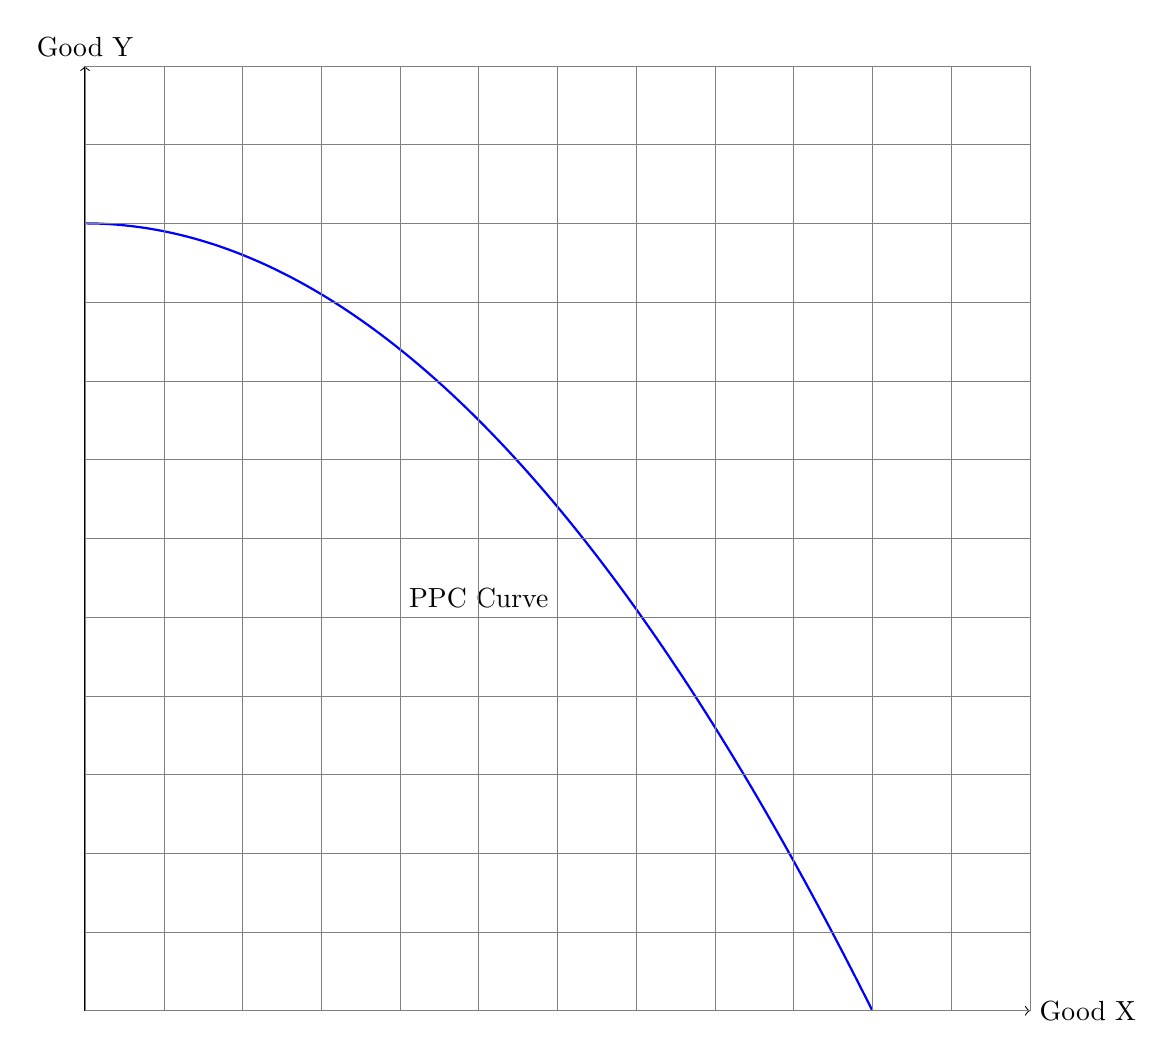
\begin{tikzpicture}
      % Draw the axes
      \draw[->] (0,0) -- (12,0) node[right] {Good X};
      \draw[->] (0,0) -- (0,12) node[above] {Good Y};
      
      % Draw the PPC curve
      \draw[thick, blue, domain=0:10] plot[variable=\x, samples=100] ({\x}, {10 - (\x^2 / 10)});
      
      % Add labels for the curve
      \node at (5, 5) [above] {PPC Curve};
      
      % Add a grid for reference
      \draw[gray, very thin] (0,0) grid (12,12);
  \end{tikzpicture} \\
  That is the curve of $100\%$ efficiency, if a business was working at the capacity of its infrastructure. Each point anywhere in the sample space presented could be the effecient, innefecient, or infeasible. If product production values are beyond the curve, they are infeasible. If inside, innefecient. There is also oppurtunity cost, where each additional unit of production has a cost in the form of the production of another simply because of the resources used.
}
\thm{Models}{
A model is any simplified version of reality used to better understand a real-life situation. In economics, it's simply applied mathematics. A PPC is also a type of model because the actual datapoints on the curve are discrete values in real life, whith more than the two dimensions presented in slice form here.
}
\dfn{What it means for an economy to be \textbf{Growing}}{An economy now has more production posibilities, as in the feasible sample space where a production possibility can be chosen from is larger. This can either be because of an increase of availability of a factor of production or better technology.}
\dfn{4 factors of production}{
\begin{itemize}
  \item labor
  \item land
  \item capital
  \item entrepreneurship
\end{itemize}
}
\subsection{ FOP, the Factors of production }
\begin{note}
  WRIP is the acronym for the income streams generated off of the factors of production. 
  \begin{itemize}
    \item land $\rightarrow$ Rent
    \item labor $\rightarrow$ wages
    \item capital $\rightarrow$ interest
    \item entrepreneurship $\rightarrow$ owner and stuff, you know
  \end{itemize}
\end{note}
\section{Friday, August 16h}
\dfn{Recession}{
  A recession is a contraction of the econmy measured by negative growth of the GDP for 3 months.
}
\dfn{Economic Growth terms}{
  An expansion is a measurable increase of the PPC boundraies through GPD and other things. Peak is the, well the peak of the growth percentages. Trough is the lowest growth percentage of the contraction cycle. During an expansion: \\
  \begin{itemize}
    \item Inflation $\uparrow$
    \item Unemployment $\downarrow$
    \item GDP $\uparrow$
    \item Inflation $\uparrow$
    \end{itemize}
  During a contraction: \\
  \begin{itemize}
    \item Inflation $\downarrow$
    \item Unemployment $\uparrow$
    \item GDP $\downarrow$
  \end{itemize}
  Think about each one and why.
}
\thm{The Fed causes recessions}{
  Here's why: to control inflation, the fed must increase intrest rates, which makes it harder for people to spend money that they don't actually have. Therefore, businesses don't make as much money, and they fire peopele and so on in a death spiral. 
}
\dfn{Inflation vs. Disinflation vs. Deflation}{
  \textbf{They're different, be careful.} Inflation is when prices go up. Disinflation is good though, it is the readjustment of the inflation rate to be lower. But when prices go down, disinflation occurs, there's less money on the table for \textit{everyone}.
}
\thm{This is why Innovation and Competition are so important.}{
  They're important because they are the \textit{secure} way to decrease the prices of goods without causing an economic death spiral. Think on it.
}
\begin{note}
This is the deal. You can't compete - in terms of prices - with another business because someone else can always outbid you. Therefore, you must act on \textit{quality}.
\end{note}
\dfn{Comparative Advantage}{
  Comparative advantage is an economy's ability to produce a particular good or service at a lower opportunity cost than its trading partners. Comparative advantage is used to explain why companies, countries, or individuals can benefit from trade.
}
\dfn{Absolute Advantage}{
  Absolute advantage is the ability of an individual, company, region, or country to produce a greater quantity of a good or service with the same quantity of inputs per unit of time, or to produce the same quantity of a good or service per unit of time using a lesser quantity of inputs, than its competitors.
}
\begin{note}
Absolute advantage only covers that Entity A can make more than Entity B. Compartive advantage is more complicated: \\
$$
\frac{\text{Entity B's import of Good Y}}{\text{Entity A's Good X} }
$$
$$
\frac{\text{Entity B's import of Good X}}{\text{Entity A's Good Y}} 
$$
$$
\frac{\text{Entity A's import of Good Y}}{\text{Entity B's Good X}}
$$
$$
\frac{\text{Entity A's import of Good X}}{\text{Entity B's Good Y}}
$$

  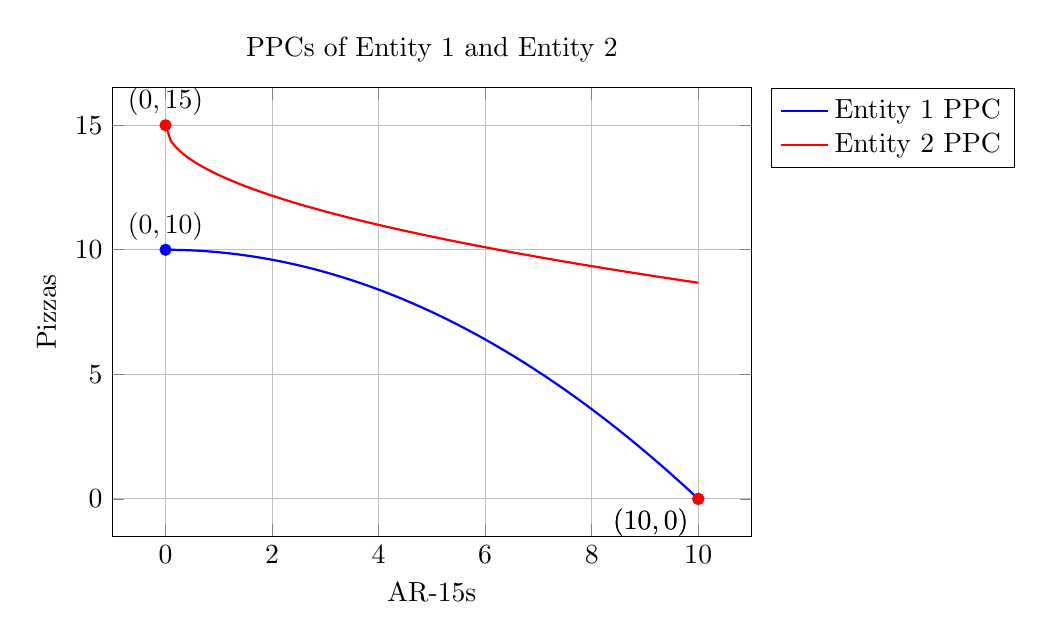
\begin{tikzpicture}
        \begin{axis}[
            width=0.8\textwidth,
            height=0.6\textwidth,
            xlabel={AR-15s},
            ylabel={Pizzas},
            title={PPCs of Entity 1 and Entity 2},
            legend pos=outer north east,
            grid=major,
            domain=0:10,
            samples=100,
            xmajorgrids=true,
            ymajorgrids=true
            ]
            % PPC for Entity 1
            \addplot[blue, thick] {10 - (x^2)/10};
            \addlegendentry{Entity 1 PPC}

            % PPC for Entity 2
            \addplot[red, thick] {15 - 2*sqrt(x)};
            \addlegendentry{Entity 2 PPC}

            % Annotate intersection points for Entity 1
            \addplot[only marks, mark=*, color=blue] coordinates {(0,10) (10,0)};
            \node at (axis cs:0,10) [anchor=south] {$(0,10)$};
            \node at (axis cs:10,0) [anchor=north east] {$(10,0)$};

            % Annotate intersection points for Entity 2
            \addplot[only marks, mark=*, color=red] coordinates {(0,15) (10,0)};
            \node at (axis cs:0,15) [anchor=south] {$(0,15)$};
            \node at (axis cs:10,0) [anchor=north east] {$(10,0)$};

            % Axis limits
            \axisline style={->};
        \end{axis}
    \end{tikzpicture}
  This is such a graph where there exists no comparative advantage because the oppurtunity cost to produce AR-15s vs. That of Pizzas is always cheaper than the \textbf{terms of trade} if Entity 1 were to trade with Entity 2. Entity A has the coimplete Absolute advantage, and has no need to work with Entity 2. However, it is important to note that Absolute advanteage does not mean that there does not exist a comparative advantage. 
  \vspace{1cm}

\begin{tikzpicture}[scale=1.2]
    % Axes
    \draw[->] (0,0) -- (11,0) node[right] {Pizzas};
    \draw[->] (0,0) -- (0,6.5) node[above] {AR-15s};
    
    % Labels for axes
    \node[below] at (10,0) {10,000};
    \node[below] at (5,0) {5,000};
    \node[left] at (0,5) {5,000};
    \node[left] at (0,1) {1,000};
    
    % PPCs
    \draw[thick, blue] (0,1) to[out=-5,in=160] (10,0) node[right] {A};
    \draw[thick, red] (0,5) to[out=-30,in=120] (5,0) node[right] {B};
    
    % Intersection point


    % Legend
    \node[blue, right] at (5.5,6) {A: Italian Military};
    \node[red, right] at (5.5,5.5) {B: American Military};
    
    % Title
    \node[above] at (5.5,6.5) {\large Intersecting Production Possibility Curves};
\end{tikzpicture}

\end{note}
\end{document}

